\documentclass[12pt,a4paper]{report}

%Set language
\usepackage[english]{babel}
\usepackage{enumerate}

% To import and adjust images
\usepackage{graphicx}
\usepackage[export]{adjustbox}
\usepackage[center]{caption}
\usepackage{subcaption}
\usepackage{float}
\usepackage{tabularx}
\usepackage{lipsum}
\usepackage{caption}
\usepackage{eurosym}
\usepackage{amssymb}

% To define custom operators
\usepackage{amsmath}
\DeclareMathOperator*{\argmax}{argmax} 

% To use monospaced font
\usepackage{courier}

% To build a clickable Toc
\usepackage{color} %May be necessary if you want to color links
\usepackage{hyperref}
\hypersetup{
    colorlinks=true, %set true if you want colored links
    linktoc=all,     %set to all if you want both sections and subsections linked
    linkcolor=black,  %choose some color if you want links to stand out
    urlcolor = black
}


%To load PoLitecnico's logo
\usepackage{titling}

% Command to hide subsections in the Toc
\setcounter{tocdepth}{1}

% I don't like dots in the Toc
\usepackage{tocloft}
\renewcommand{\cftdot}{}

%To improve the tables
\usepackage[table]{xcolor}

%To break line inside tables
%\usepackage[utf8]{inputenc}
%\usepackage{fourier} 
%\usepackage{array}
\usepackage{makecell}
%\renewcommand\theadalign{bc}
%\renewcommand\theadfont{\bfseries}
\renewcommand\theadgape{\Gape[4pt]}

% Path relative to the .tex file containing the \includegraphics command
\graphicspath{ {./images/} }

% To change the ToC title
\addto\captionsenglish{ \renewcommand {\contentsname} {Table of contents}}
 
%logo
\pretitle{
	 \begin{center}
	 \LARGE
	 
\includegraphics[width = 0.6\textwidth]{logo}\\[\bigskipamount]
}
\posttitle{\end{center}}

% Here we go
\title{Data Intelligence Applications Homework}
\author{D'Amato Francesco - 10560062 - 945814, \\
	Frantuma Elia - 10567359 - 945729, \\
	Fucci Tiziano - 10524029 - 946638}
\date{A.Y. 2020/2021}

\begin{document}
	\maketitle
	%Index
	\tableofcontents
	\chapter{Introduction}
		\section{Scenario}
			Consider the scenario in which advertisement is used to attract users on an ecommerce website and the users, after the purchase of the first unit of a consumable item, will buy additional units of the same item in future. The goal is to find the best joint bidding and pricing strategy taking into account future purchases.

\begin{figure}[H]
\centering
  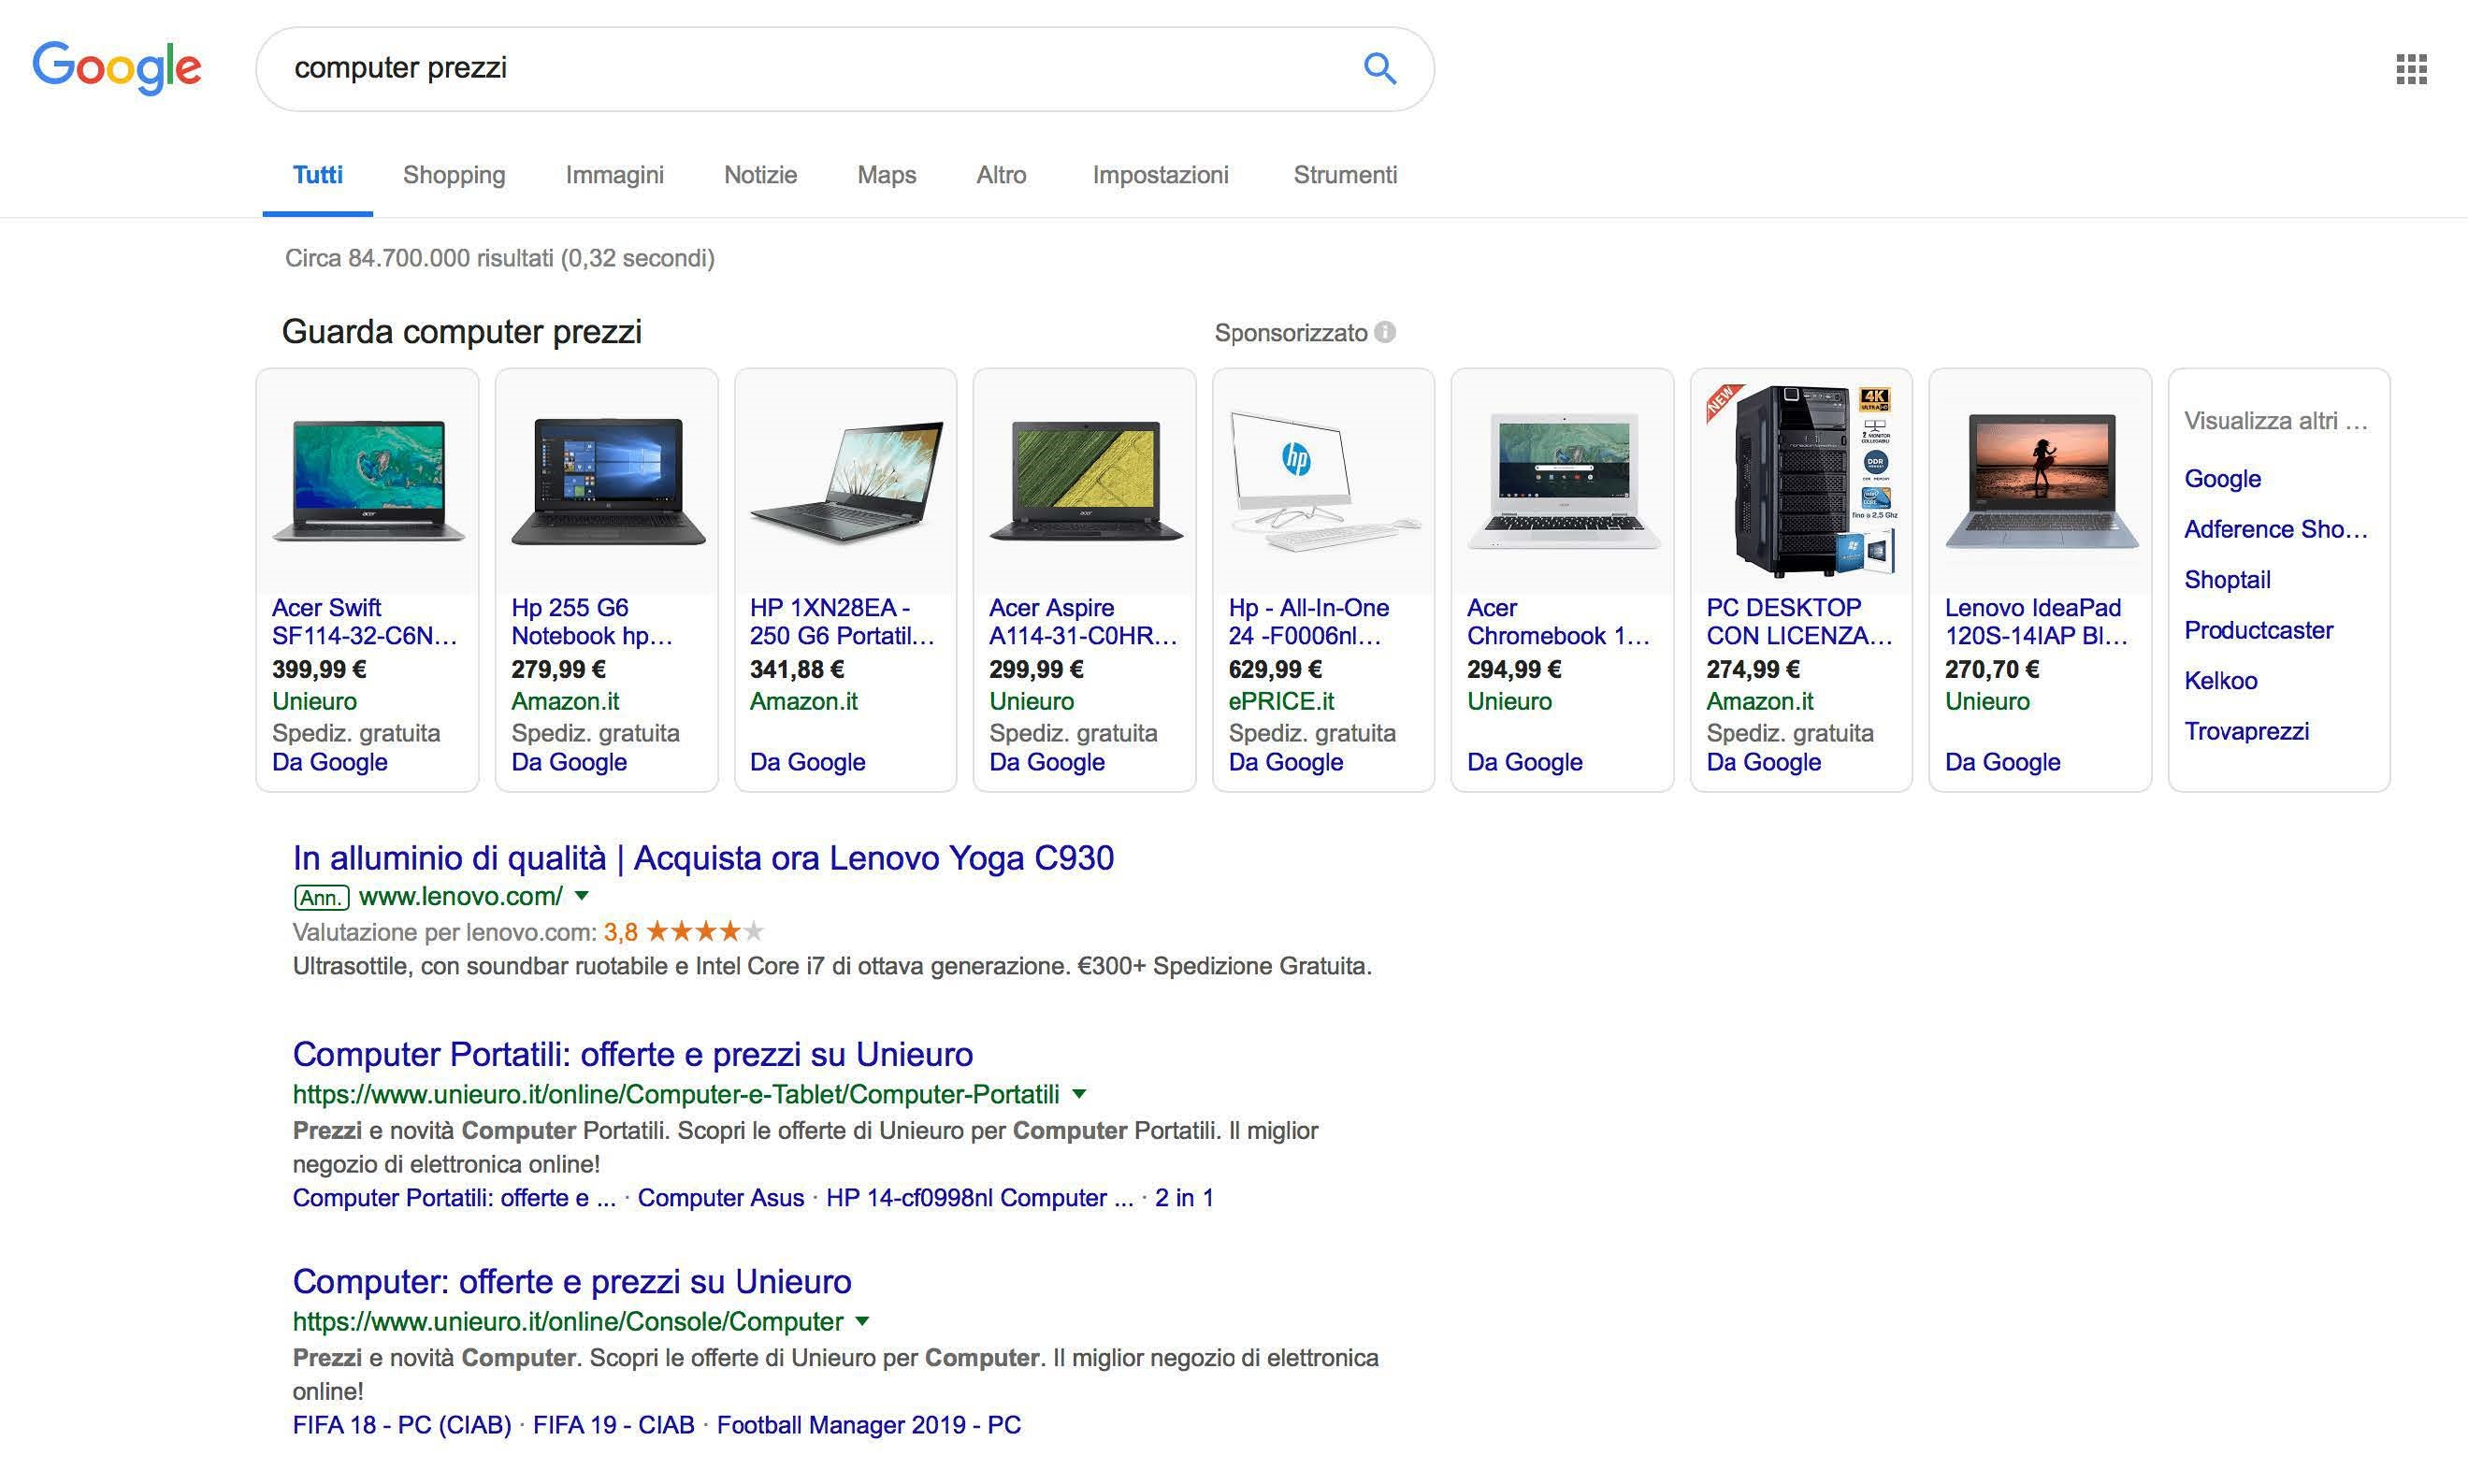
\includegraphics[scale = 0.3, center]{image0}
  \caption{Advertising example}
\end{figure}

\section{The product}
The product we have chosen to simulate this advertising scenario is an energy drink. As we will say later, the first unit of product comes with a "dash button", to encourage the customer to buy it again and simulate the re-buy process.
\begin{figure}[H]
\centering
  
\includegraphics[scale = 0.7, center]{redbull-dash}
  \caption{The sold product}
\end{figure}
	%end of first chapter

	\chapter{Environment}		
In this section we give a precise definition of the customer classes and their features, cost functions and distribution probabilities on which the model is based.

		\section{Customers classes}
In the environment model we have three customer classes: C1, C2 and C3.
They represent customers with different needs, age and tastes and thus different interest in buying the product.

			\subsection{Class 1: the sportsman}
The first class is composed by people who play sports or train regularly. They are interested in buying the energy drink to improve their performance. 


Their conversion rate function is: 
\[ \mathcal C_1(p) =  1.4 e^{-0.14p}\]
\begin{figure}[H]
\centering
  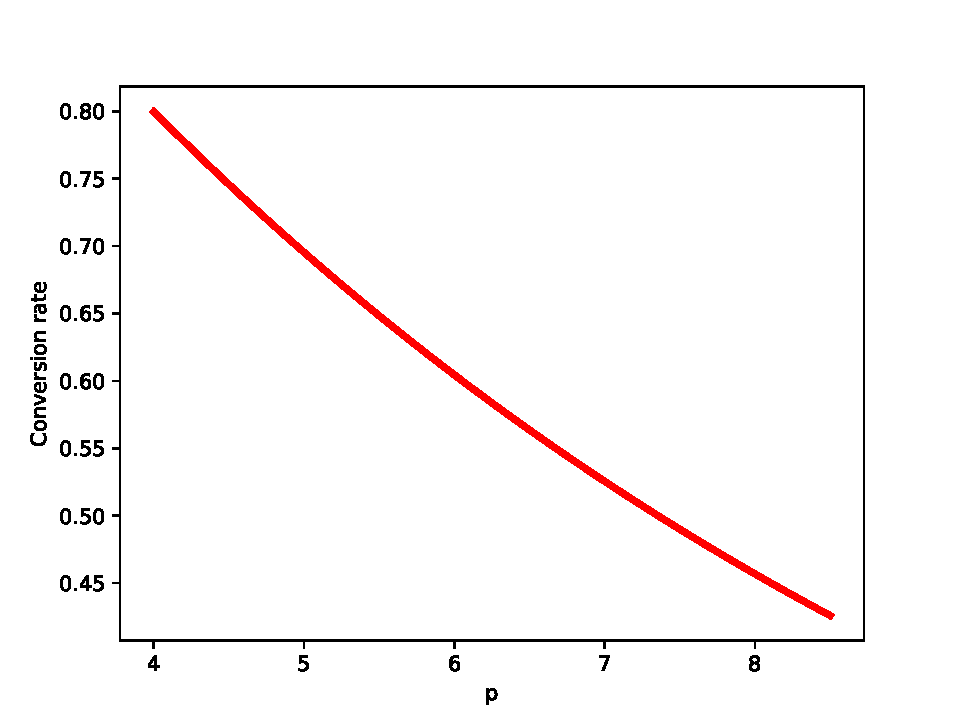
\includegraphics[scale = 0.8, center]{C1}
  \caption{Conversion rate function of Class 1.}
\end{figure}

and the number of purchases following the first one is described by: 
\[X \sim  \mathcal{P}oisson   (\lambda),\] where:
\[\lambda = \frac{4.0}{\frac p 5 +0.5}  \]

			\subsection{Class 2: the retired man}
The average members of this class buy the product just to enjoy its taste.

Their conversion rate function is: 
\[ \mathcal C_2(p) = 0.1+ 6 e^{-0.6p}\]
\begin{figure}[H]
\centering
  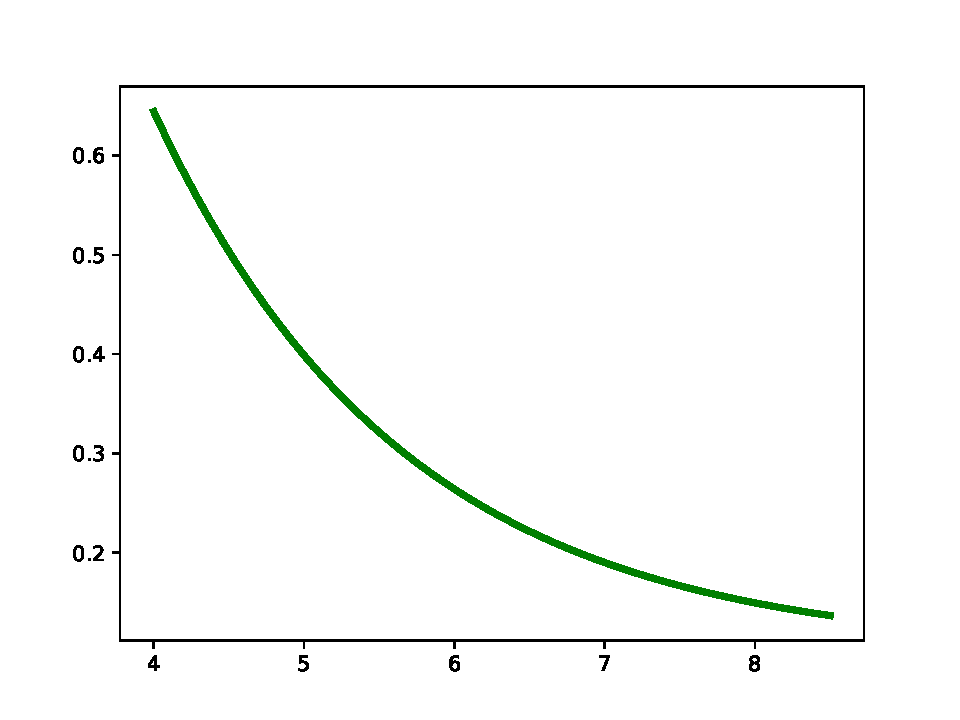
\includegraphics[scale = 0.8, center]{C2}
  \caption{Conversion rate function of Class 2.}
\end{figure}

and the number of purchases following the first one is described by: 
\[X \sim  \mathcal{P}oisson   (\lambda),\] where:
\[\lambda = \frac{2.0}{\frac p 5 +0.5}  \]

			\subsection{Class 3: the programmer}
Programmers need to stay focused for a long time while at work, so they are interested in buying the product to work better and avoid introducing bugs in the code.


Their conversion rate function is: \[   \mathcal C_3(p) = \left\{
\begin{array}{ll}
      0.8 e^{-0.5(p-5.5)^2} & 4.0\leq p< 6 \\
      20 e^{-0.557p} & p \geq 6 \\
\end{array} 
\right. \]
\begin{figure}[H]
\centering
  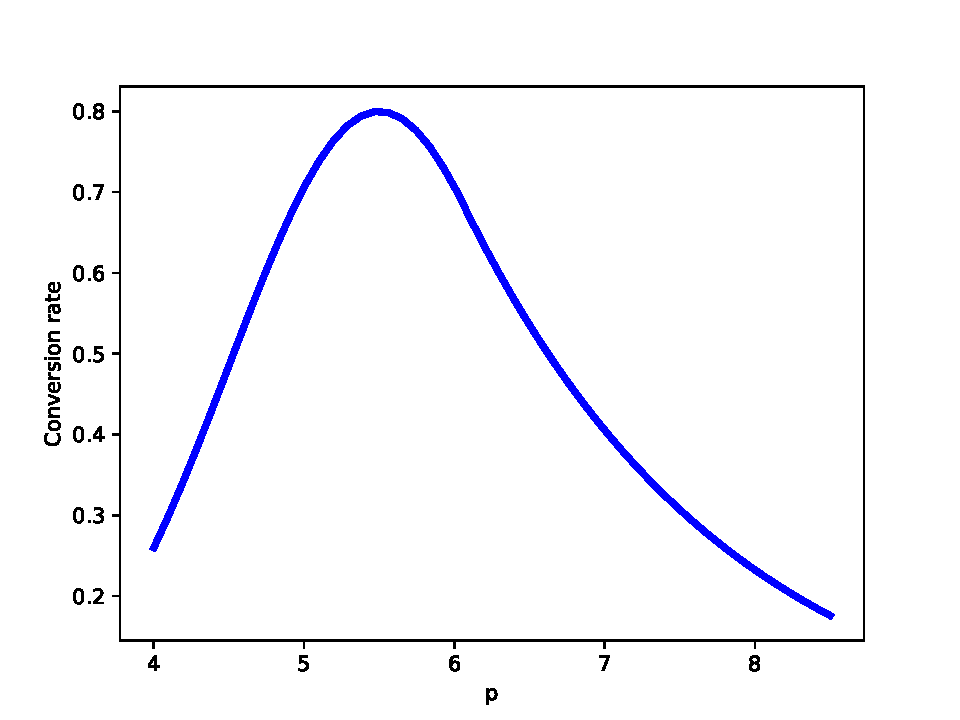
\includegraphics[scale = 0.8, center]{C3}
  \caption{Conversion rate function of Class 3.}
\end{figure}


and the number of purchases following the first one is described by: 
\[X \sim  \mathcal{P}oisson   (\lambda),\] where:
\[\lambda = \frac{3.0}{\frac p 5 +0.5}  \]


		\section{Advertising}

			\subsection{Auctions}
In our model, we make the hypothesis of a GSP (Generalized Second Price) auction mechanism:
	\[p_a= \frac{q_a}{q_{a+1}}v_{a+1} \left( \leq\frac{q_a}{q_a}v_a = v_a\right)\]
However, since we are not required to model the other auctionists, we make the following simplification:
	\[  p_a = v_a - |X|\] 
where $ X\sim \mathcal{N}(\mu,\,\sigma^{2})$ having $\mu = \frac{v_a}{10} ,\,\sigma^{2} = 0.1$,
that is assuming that we are generally paying for $\frac 9 {10}$ of our bid. The random variable $p_a$ represents the stochastic cost per click.

			\subsection{Daily clicks of new users}
The number of daily clicks of new users of class $\mathcal C_i$ is a random variable drawn from a Gaussian distribution:
\[ X_i\sim \mathcal{N}(\mu_i,\,\sigma^{2})\]
If the task requires to find the optimal bidding strategy, we model the influence of the bid on the number of daily clicks:
\[ X_i \sim \mathcal{N}(\mu_{0,i}+\mu_{bid,i},\,\sigma^{2})\]
where $\mu_{0,i}$ is a fixed value and $\mu_{bid,i}$ is an increment which grows monotonically with the bid.

			\subsection{Conversion rate functions}
The conversion rate functions are defined for each class as the probability that the user of that class will buy the product at a given price. In particular, we have:
\[ \mathcal C_1(p) =  1.4 e^{-0.14p}    \]
\[ \mathcal C_2(p) = 0.1+ 6 e^{-0.6p}    \]
\[   \mathcal C_3(p) = \left\{
\begin{array}{ll}
      0.8 e^{-0.5(p-5.5)^2} & 4.0\leq p< 6 \\
      20 e^{-0.557p} & p \geq 6 \\
\end{array} 
\right. \]
\[ \mathcal C_{agg}(p, b) =\frac{n_1(b)\mathcal C_1(p)+n_2(b)\mathcal C_2(p)+n_3(b)\mathcal C_3(p)}{n_1(b)+n_2(b)+n_3(b)}\] 
where $n_i$ is the population of Class $i$ and the coefficients $n_i(b)$ are function of the bid.
Since in our model $4.00 \leq p \leq 8.50$, $\mathcal C_i(p) \in [0,1]$ $ \forall i$.
\begin{figure}[H]
\centering
  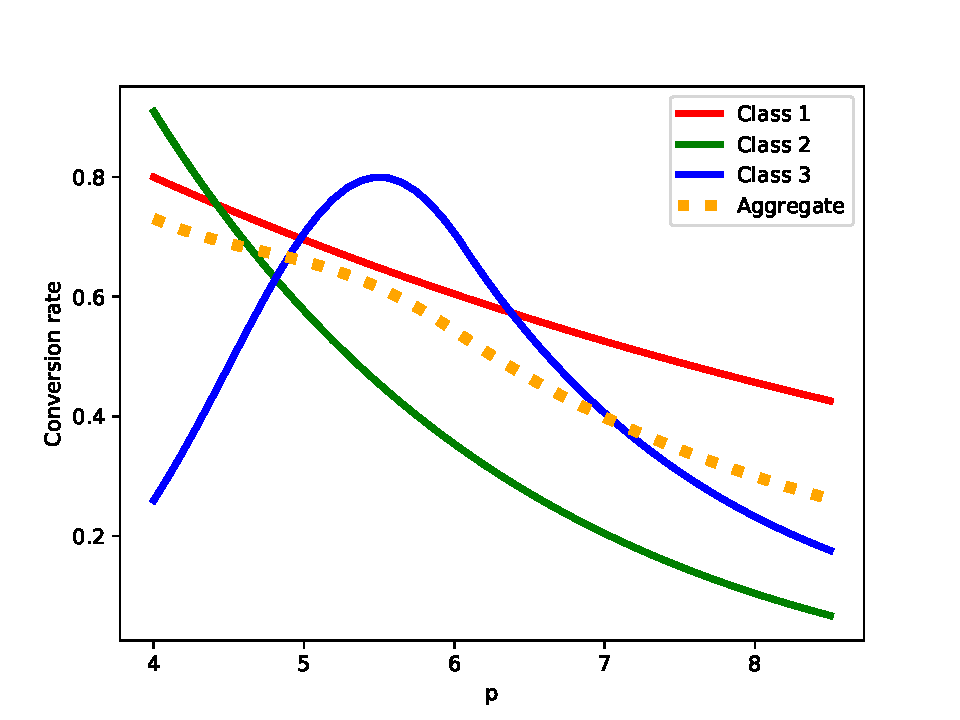
\includegraphics[scale = 0.8, center]{Cagg}
  \caption{Conversion rate function of the aggregate Class, obtained for a fixed bid $b=2,50$\euro.}
\end{figure}



		\section{Re-buy process}
We modeled the re-buy process as the orders the customer makes using a dash button, which comes for free together with the first bought item. We assume that the price of the additional purchases is the same of the first one.
The number of purchases (following the first one) that a customer of Class $i$ makes in one month is modeled as a random variable with a Poisson probability distribution:
\[X_i \sim  \mathcal{P}oisson   (\lambda_i) \]
where the parameter $\lambda_i$ is function of the price: $\lambda_i(p) = \frac{\alpha_i}{\beta_i(p+k_i)}$, with $\alpha_i, \beta_i$ and $k_i$ normalizing constants.
For the aggregate model:
\[\lambda_{agg}(p,b) =\frac{n_1(b)\lambda_1(p)+n_2(b) \lambda_2(p)+n_3(b) \lambda_3(p)}{n_1(b)+n_2(b)+n_3(b)} \] The following diagram shows the behaviour of $X_i$ as the price increases:
\begin{figure}[H]
\renewcommand*\thesubfigure{\roman{subfigure}} 
\centering
\begin{subfigure}{.49\textwidth}
  \centering
  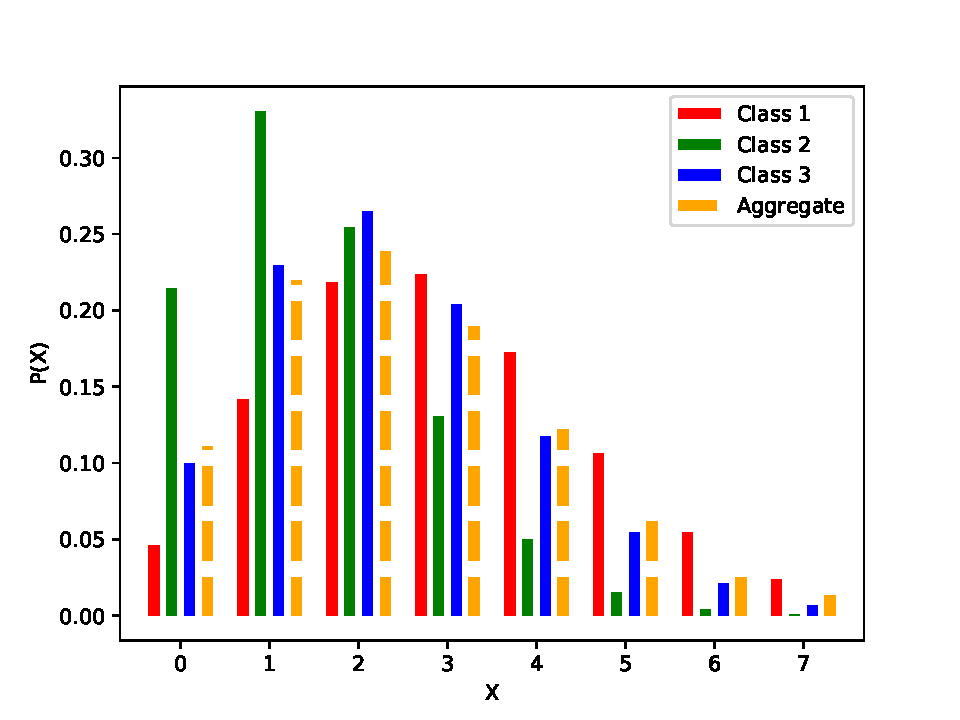
\includegraphics[width=1\linewidth]{4e}
  \caption{p = 4\euro}
  \label{fig:sub1}
\end{subfigure}
\begin{subfigure}{.49\textwidth}
  \centering
  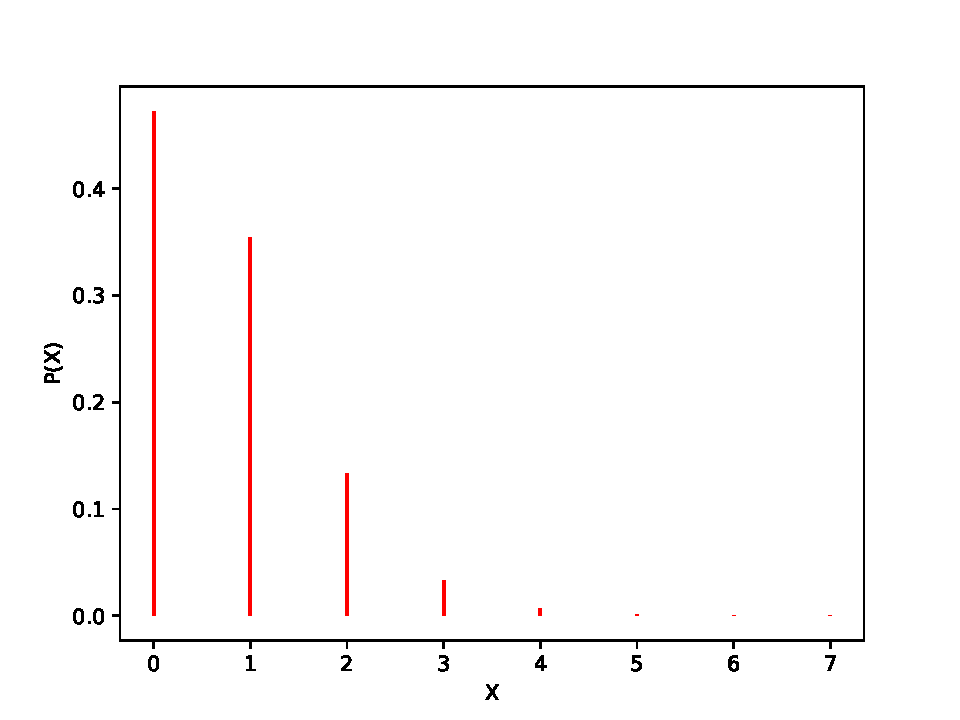
\includegraphics[width=1\linewidth]{55e}
  \caption{p = 5.5\euro}
  \label{fig:sub2}
\end{subfigure}
\begin{subfigure}{.49\textwidth}
  \centering
  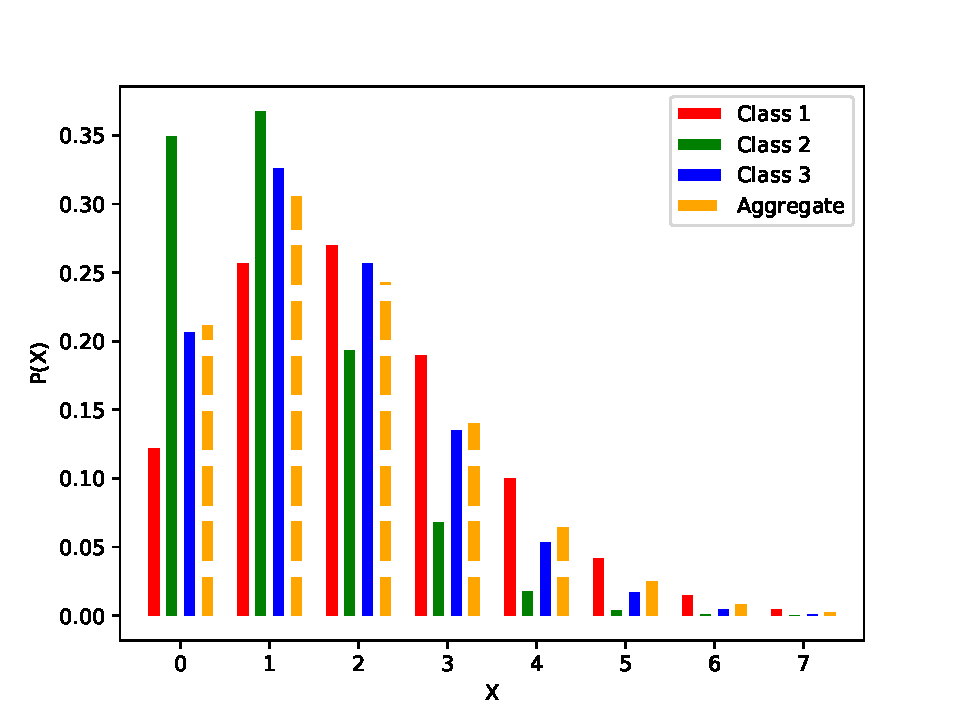
\includegraphics[width=1\linewidth]{7e}
  \caption{p = 7\euro}
  \label{fig:sub3}
\end{subfigure}
\begin{subfigure}{.49\textwidth}
  \centering
  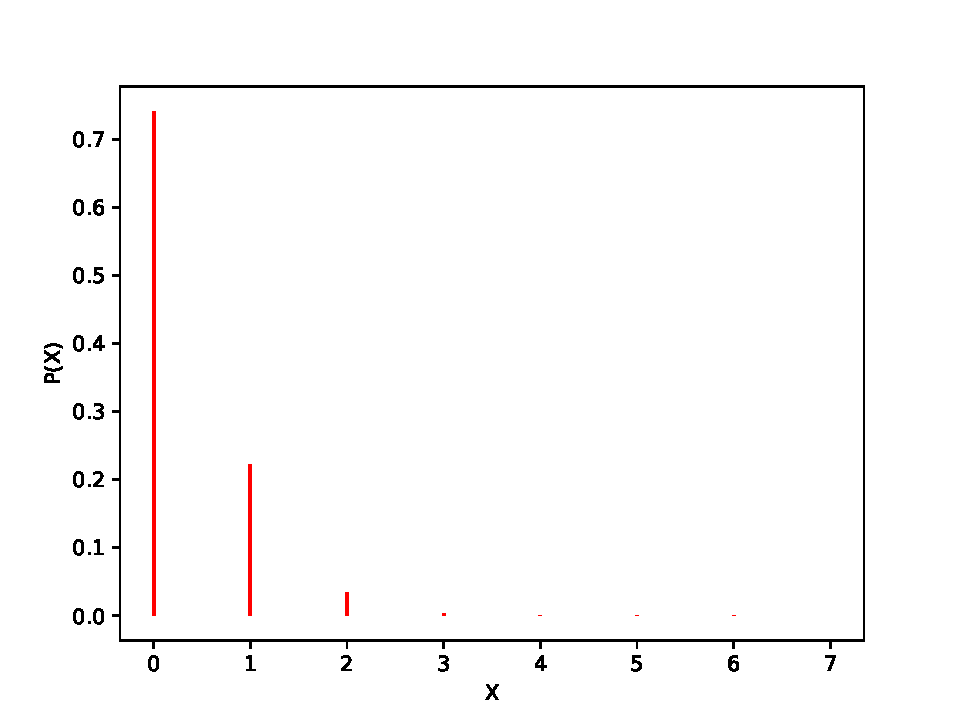
\includegraphics[width=1\linewidth]{85e}
  \caption{p = 8.5\euro}
  \label{fig:sub4}
\end{subfigure}
	\caption{Poisson distributions for the three Classes and the aggregate Class, obtained for different prices and a fixed bid $b=2,50$\euro.}
\end{figure}

	%end of second chapter

	\chapter{Assignments}
		\section{Step 1}
			\subsection{Task}
\textit{Formulate the objective function when assuming that, once a user makes a purchase with a price p, then the ecommerce will propose the same price p to future visits of the same user and this user will surely buy the item. The revenue function must take into account the cost per click, while there is no budget constraint. Provide an algorithm to find the best joint bidding/pricing strategy and describe its complexity in the number of values of the bids and prices available (assume here that the values of the parameters are known). In the following steps, assume that the number of bid values are 10 as well as the number of price values.}
			\subsection{Solution}

		\section{Step 2}
			\subsection{Task}
\textit{Consider the online learning version of the above optimization problem when the parameters are not known. Identify the random variables, potential delays in the feedback, and choose a model for each of them when a round corresponds to a single day. Consider a time horizon of one year.}
			\subsection{Solution}

		\section{Step 3}
			\subsection{Task}
\textit{Consider the case in which the bid is fixed and learn in online fashion the best pricing strategy when the algorithm does not discriminate among the customers’ classes (and therefore the algorithm works with aggregate data). Assume that the number of daily clicks and the daily cost per click are known. Adopt both an upper-confidence bound approach and a Thompson-sampling approach and compare their performance.}
			\subsection{Results}

\begin{figure}[H]
\centering
  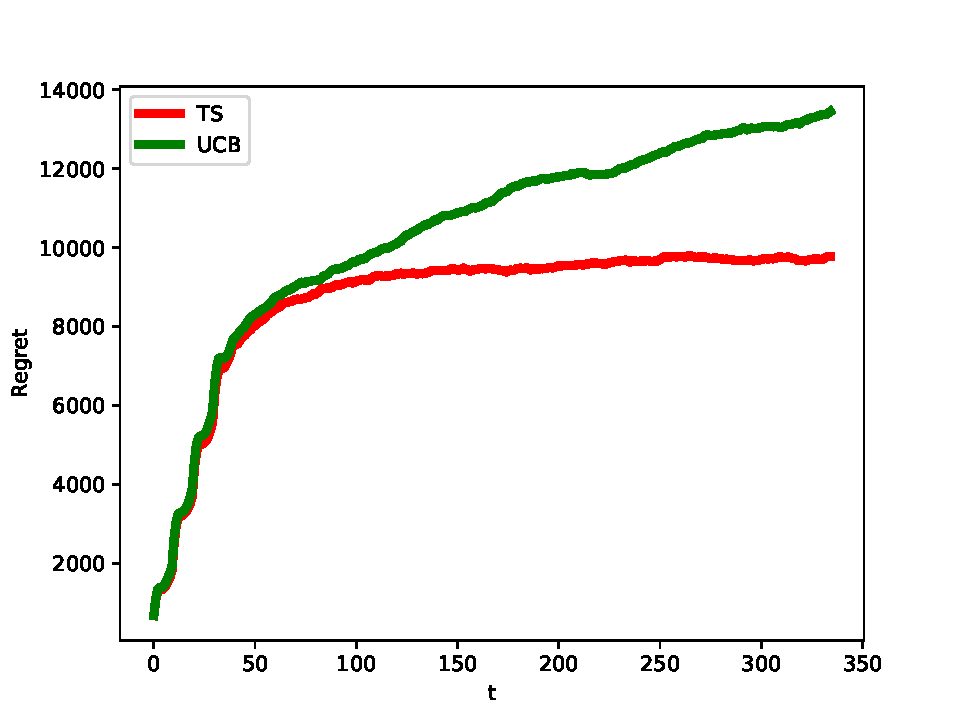
\includegraphics[scale = 0.8, center]{3r}
  \caption{Regret plots of both TS and UCB algorithms.}
\end{figure}
\begin{figure}[H]
\centering
  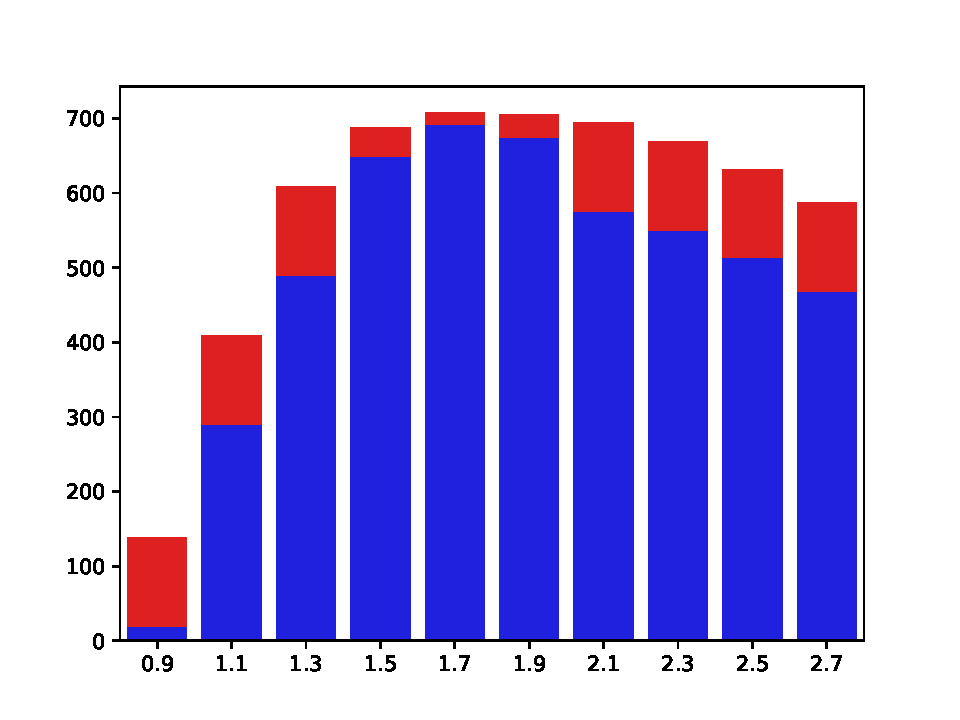
\includegraphics[scale = 0.8, center]{3ucb}
  \caption{Estimated rewards for each arm and relative upper bounds.}
\end{figure}
\begin{figure}[H]
\centering
  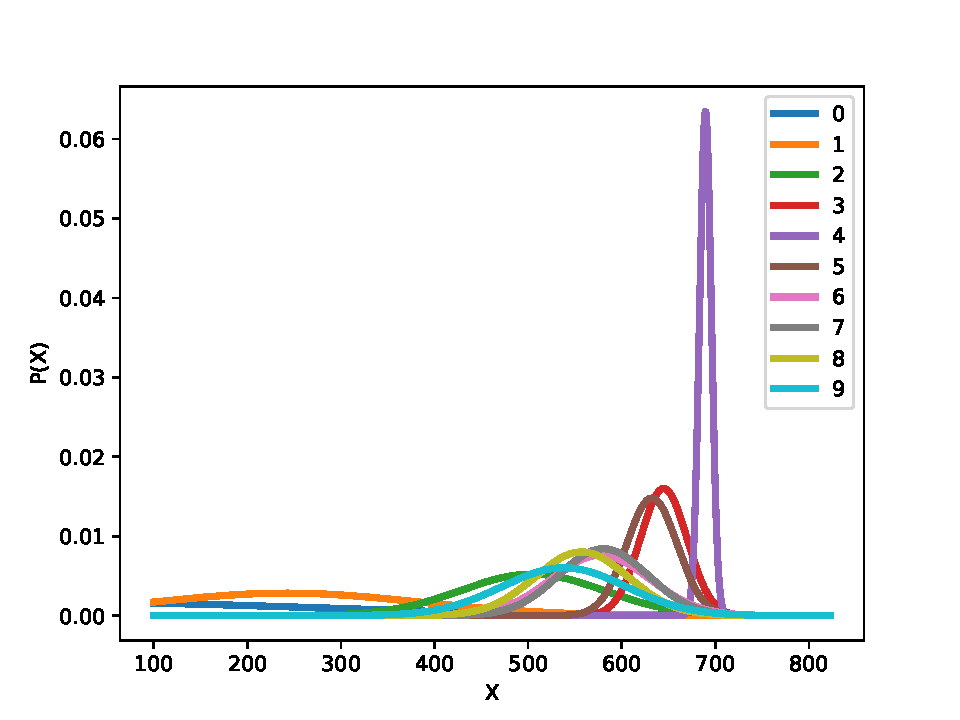
\includegraphics[scale = 0.8, center]{3arms}
  \caption{Posterior distribution over the arms reward obtained by TS.}
\end{figure}

		\section{Step 4}
			\subsection{Task}
\textit{Do the same as step 3 when instead a context-generation approach is adopted to identify the classes of customers and adopt a potentially different pricing strategy per class. In doing that, evaluate the performance of the pricing strategies in the different classes only at the optimal solution (e.g., if prices that are not optimal for two customers’ classes provide different performance, you do not split the contexts). Let us remark that no discrimination of the customers’ classes is performed at the advertising level. From this step on, choose one approach between the upper-confidence bound one and the Thompson-sampling one.}
			\subsection{Results}
		\section{Step 5}
			\subsection{Task}
\textit{Consider the case in which the prices are fixed and learn in online fashion the best bidding strategy when the algorithm does not discriminate among the customers’ classes. Assume that the conversion probability is known. However, we need to guarantee some form of safety to avoid the play of arms that provide a negative revenue with a given probability. This can be done by estimating the probability distribution over the revenue for every arm and making an arm eligible only when the probability to have a negative revenue is not larger than a threshold (e.g., 20\%). Apply this safety constraint after 10 days to avoid that the feasible set of arms is empty, while in the first 10 days choose the arm to pull with uniform probability. Do not discriminate over the customers’ classes.}
			\subsection{Results}

\begin{figure}[H]
\centering
  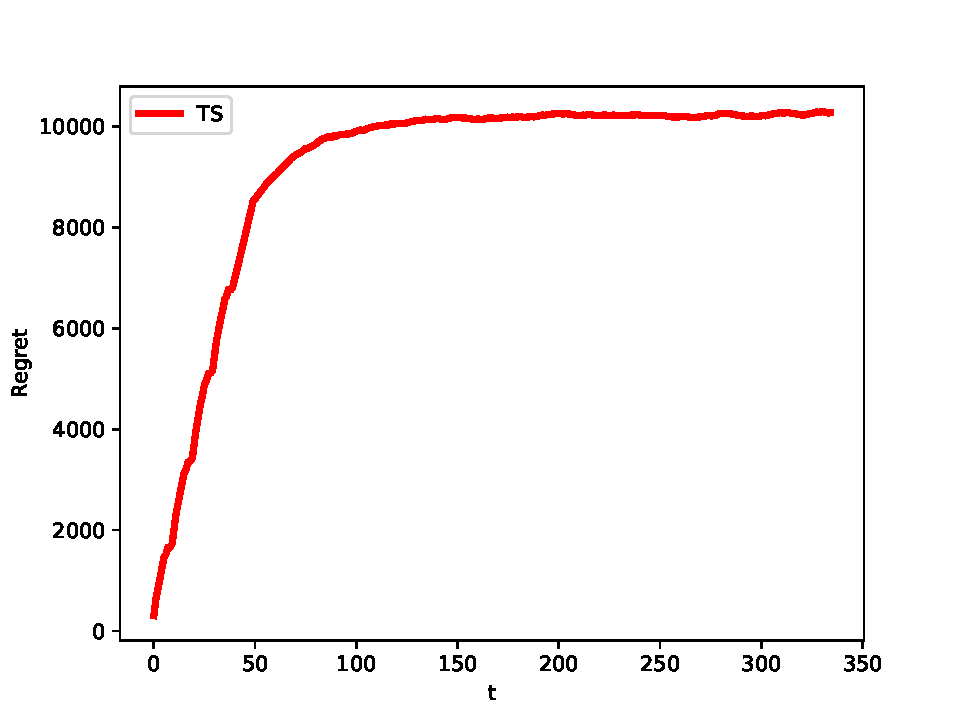
\includegraphics[scale = 0.8, center]{5r}
  \caption{Regret plots of the Thompson Sampling algorithm.}
\end{figure}
\begin{figure}[H]
\centering
  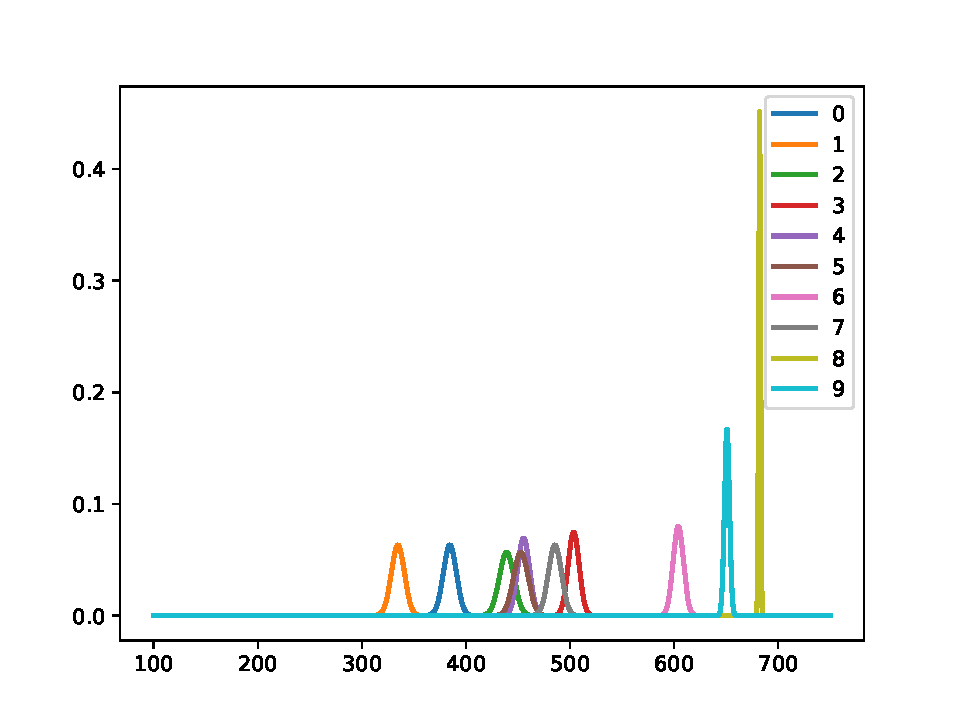
\includegraphics[scale = 0.8, center]{5arms}
  \caption{Posterior distribution over the arms rewards obtained by TS.}
\end{figure}
		\section{Step 6}
			\subsection{Task}
\textit{Consider the general case in which one needs to learn the joint pricing and bidding strategy under the safety constraint introduced in step 5. Do not discriminate over the customers’ classes both for advertising and pricing.}
			\subsection{Results}

\begin{figure}[H]
\centering
  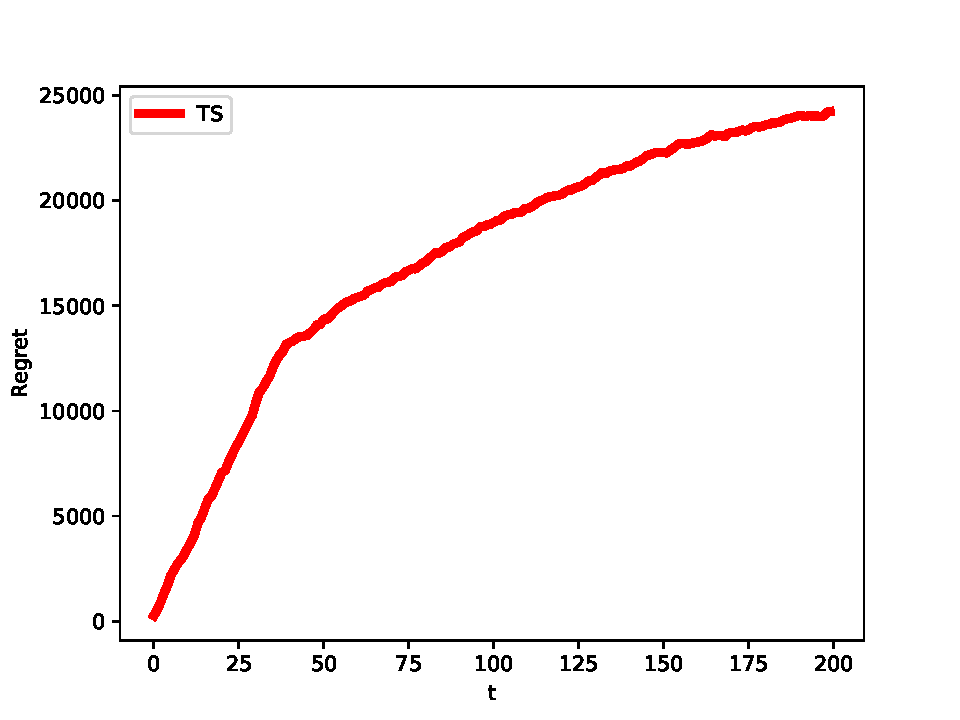
\includegraphics[scale = 0.8, center]{6r}
  \caption{Regret plot of the GPTS algorithm.}
\end{figure}
\begin{figure}[H]
\centering
  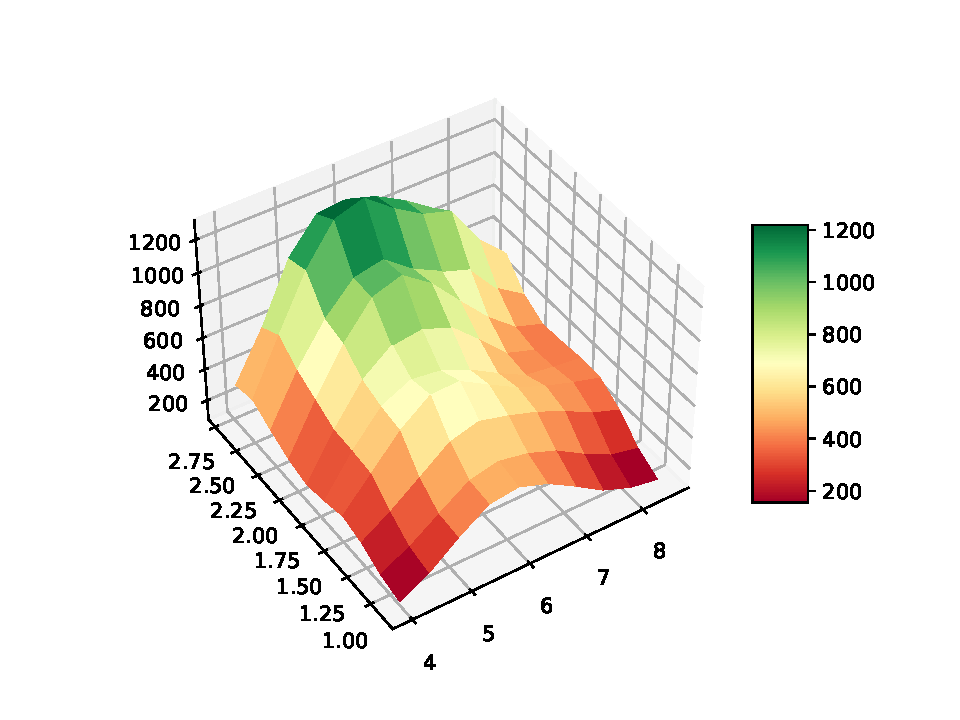
\includegraphics[scale = 0.8, center]{6arms}
  \caption{Posterior distribution over the arms rewards obtained by GPTS.}
\end{figure}
		\section{Step 7}
			\subsection{Task}
\textit{Do the same as step 6 when instead discriminating over the customers’ classes for pricing. In doing that, adopt the context structure already discovered in step 4.}
			\subsection{Results}
	%end of third chapter

	\chapter{Algorithms and other details}
		\section{UCB}
Step 3 requires to adopt an upper-confidence bound approach. The algorithm we use is a slightly modified version of the UCB1 algorithm working on $|A|=10$ arms:
\begin{enumerate}[i)]
	\item play the arm $a=t$  $\%$  $|A|$ for the first $|A|+30$ timesteps;
	\item at timestep $t$ play arm $a_t$ such that:
		$$a_t \leftarrow \argmax_{a \in A} \left\{\bar x + 150 \sqrt{\frac{2 \log(t+1)}{n_a(t-1)}}\right\} $$
TODO: CHECK THIS
\end{enumerate}
where $n_a(t-1)$ is the number of times arm $a$ has been pulled before timestep $t$. The factor 150 is a normalizing constant, since the original expression of the UCB1 algorithm bound comes from the Hoeffding bound, which is made to estimate the expected value of a random variable with support in [0,1]. Since the rewards have much larger values, we need to adjust the respective upper bound on their expected value.

The regret of the UCB algorithm is: \\TODO: INSERT EXPRESSION


		\section{Thompson Sampling}
For steps 3, 4 and 5 we follow the Thompson approach.
Our implementation of the Thompson Sampling algorithm takes into account the Gaussian nature of the reward per each arm, since the number of new customers is a Gaussian random variable, given the bid and the price. For this reason, the prior distribution is still Gaussian. 
Except for the prior updates, the procedure is similar to the one used for Bernoulli variables:
\\TODO: CHECK CORRECTNESS
\begin{enumerate}[i)]
	\item model the prior distributions: $$\mathbb{P}(\mu_a = \theta_a) = \mathcal{N}(\theta_a, \sigma^2_a)$$
	\item initialize the posterior distributions: $$\mathbb{P}(X|\mu_{0,a}, \tau_{0,a}) = \mathcal{N}(X|\mu_{0,a}, \tau_{0,a}) $$
	\item at every time $t$, for every arm $a$:
\[ \tilde \theta_a \leftarrow Sample\left(\mathbb{P}(\mu_a = \theta_a)\right)\]
	\item at every time $t$ play arm $a_t$ such that:
		$$a_t \leftarrow \argmax_{a \in A} \{\tilde \theta_a\} $$
	\item update the Gaussian distribution of arm $a_t$ as:
		$$\tau_{0,a} \leftarrow \tau_{0,a} + n_a(t-1)\tau_a $$
		$$\mu_{0,a} \leftarrow \frac{\tau_{0,a}\mu_{0,a} + \tau_a \sum_{i=1}^{n}{x_i}}{\tau_{0,a} + n_a(t)\tau_a} $$
\end{enumerate}
where:
\begin{itemize}
	\item $\tau_a = 1/\sigma^2_a$ is the precision of the prior distribution;
	\item $n_a$ is the number of times the arm has been pulled;
	\item $x_i$ is the reward received at each round the arm was pulled;
	\item $\mu_{0,a}$ is the estimated mean of arm $a$;
	\item $\tau_{0,a}$ is the precision of the output model.
\end{itemize}		

\section{Gaussian Process Thompson Sampling}



	%end of fourth chapter
	\chapter{References}
		\section{Links}

\begin{itemize}
	\item GitHub repository of the project: \url{https://github.com/tizianofucci/DIA2021AdvertisingAndPrincing}
	\item Application of Gaussian Thompson Sampling: \url{https://towardsdatascience.com/thompson-sampling-fc28817eacb8}
\end{itemize}

\end{document}
